%\documentclass[a4paper,twocolumn]{article} % Document type
%       Compiler: pdflatex

\documentclass[a4paper,12pt,oneside,onecolumn]{article} % Document type

\usepackage[left=1.0in, right=1.0in, top=1.0in, bottom=1.0in]{geometry}

\ifx\pdfoutput\undefined
    %Use old Latex if PDFLatex does not work
   \usepackage[dvips]{graphicx}% To get graphics working
   \DeclareGraphicsExtensions{.eps} % Encapsulated PostScript
 \else
    %Use PDFLatex
   \usepackage[pdftex]{graphicx}% To get graphics working
   \DeclareGraphicsExtensions{.pdf,.jpg,.png,.mps} % Portable Document Format, Joint Photographic Experts Group, Portable Network Graphics, MetaPost
   \pdfcompresslevel=9
\fi

\usepackage{amsmath,amssymb}   % Contains mathematical symbols
\usepackage[ansinew]{inputenc} % Input encoding, identical to Windows 1252
\usepackage[english]{babel}    % Language
\usepackage[square,numbers]{natbib}     %Nice numbered citations
\usepackage{siunitx}
\usepackage{graphicx}
\usepackage{float}
\bibliographystyle{plainnat}            %Sorted bibliography



\begin{document}               % Begins the document

\title{Homework 3 in EL2450 Hybrid and Embedded Control Systems}
\author{
  Martin Favre \\ 19920130-0010 \\ mfavre@kth.se 
  \and 
  Adam Lang \\ 19861110-3956 \\ adamlang@kth.se
  \and
  Andreas Fr�derberg \\ 19880730-7577 \\ andfro@kth.se
  \and
  }
%\date{2010-10-10}             % If you want to set the date yourself.

\maketitle                     % Generates the title


\section*{Task 1}


Given the equations 
	\begin{equation}
		u_\omega = \frac{u_r + u_l}{2}
	\end{equation}
	\begin{equation}
		u_\Psi = u_r-u_l,
	\end{equation}
and $u_\omega$ and $u_\Psi$, then $u_r$ and $u_l$ can be calculated as
	\begin{equation}
		u_r = u_\omega + \frac{u_\Psi}{2}
	\end{equation}
	\begin{equation}
		u_l =  u_\omega-\frac{u_\Psi}{2}
	\end{equation}
	
\section*{Task 2}

Using the generated data from Forward.csv and Rotate.csv, it is possible
to determine R and L. The data that is recieved, is time $[\mu$$s]$,
position x $[m]$, position y $[m]$ and rotation $\theta$$[^{\circ}]$.
%#JobbigasteTecknet2016

$\dot{x}$, $\dot{y}$ and $\dot{\theta}$ is calculated discretely. With
$R_1$ and $R_2$ and the input $\dot{x}$ and $\dot{y}$
as,
	\begin{equation}
		R_1 = \frac{\dot{x}}{cos(\theta)u_\omega}
	\end{equation}
	\begin{equation}
		R_2 = \frac{\dot{y}}{sin(\theta)u_\omega}
	\end{equation}
We can calculate $R$ as the mean value,
	\begin{equation}
		R = \frac{R_1 + R_2}{2}. % Övertydligt
	\end{equation}
L is determined simularily by calculating the mean values of from all
$\dot{\theta}$ with,
	\begin{equation}
		L =  \frac{R}{\dot{\theta}}u_\Phi
	\end{equation}
        Calculating these mean values will result in
	\begin{align*}
          &R = 5.2\ \si{\milli\meter} \\
          &L = 25.5\ \si{\milli\meter/\ang{1}}
	\end{align*}

\section*{Task 3}
        Asymptotic stability means that starting points close to the
        equilibrium point will push the system towards the same equilibrium point.
        Since this is the case for our system, we can say that is it
        asymptotically stable.
	Zeno behaviour is defined as an infinite amount of state
        transitions in a finite amount of time. This is not valid in
        this case since 
        \begin{equation}
          \lim_{l \to \infty}\sum\limits_{l=1}^\infty t_i(s_i) \neq k
        \end{equation}
        where $s$ is a state transition, $t(s)$ is the function of the time 
        for each state transitions and k is a constant.
        This can also be seen in Figure \ref{fig:task3_plot}.
        \begin{figure}[H]
        \centering
        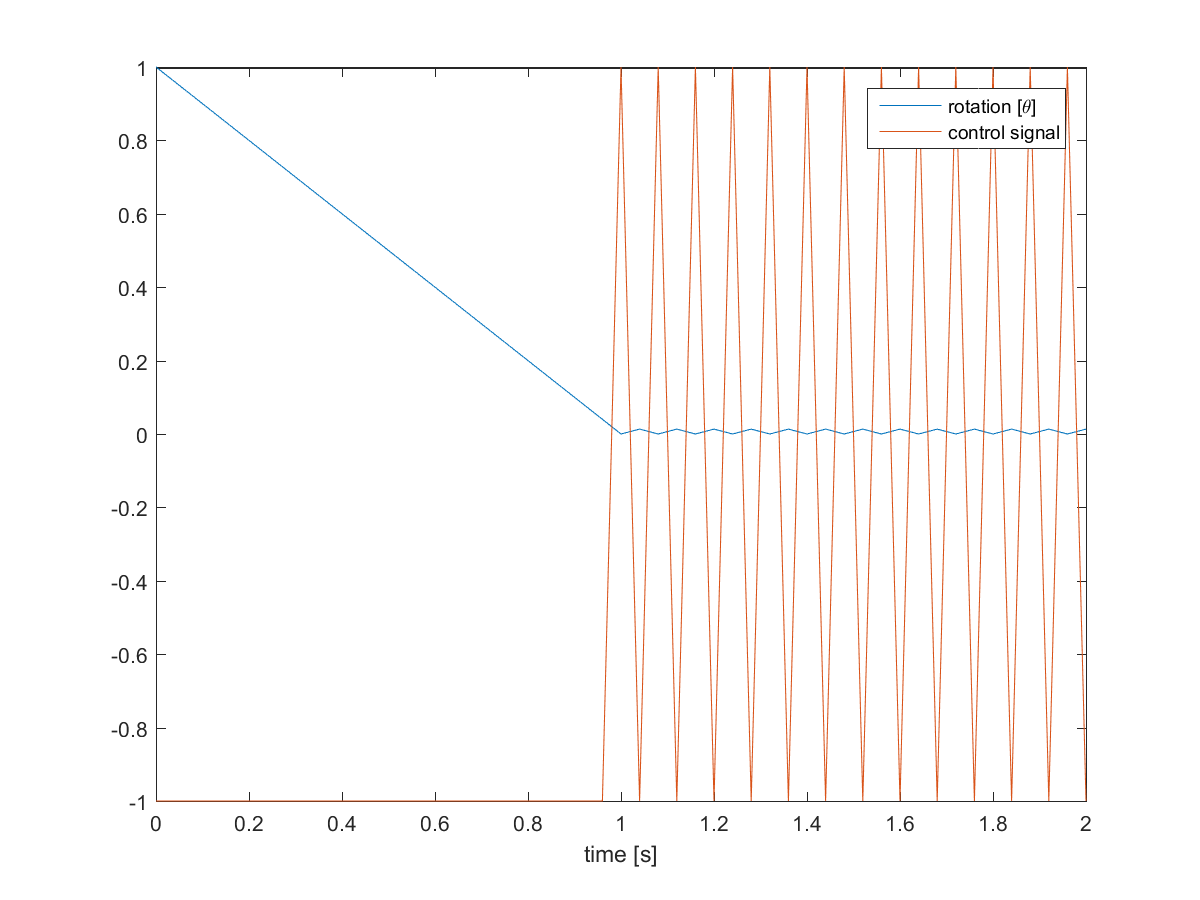
\includegraphics[scale=0.5]{../matlab/images/task3_plot.png}
        \caption{Response of rot1 simulink model.}
        \label{fig:task3_plot}
    \end{figure}

\section*{Task 4}
        Using the same definition as Task 3, we can say that the system
        is asymptotically stable and in fact does exhibit Zeno
        behaviour. In figure \ref{fig:task3_plot} the systems state
        transitions approach infinite transitions in a finite amount of
        time. 
	\begin{figure}[H]
        \centering
        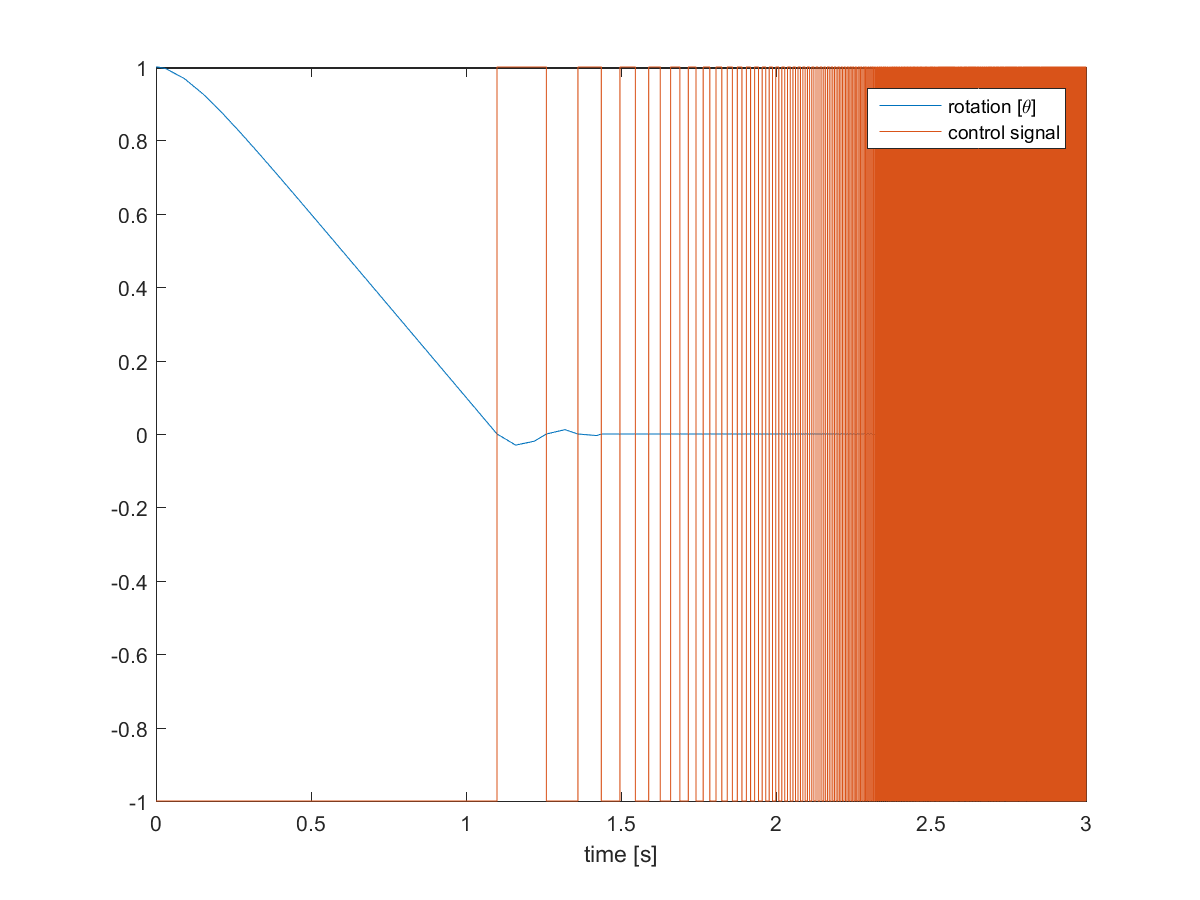
\includegraphics[scale = 0.5]{../matlab/images/task4_plot.png}
        \caption{Response of rot1 simulink model.}
        \label{fig:task4_plot}
    \end{figure}

\section*{Task 5}

	The system is stable, but not asymptotically, and does not exhibit Zeno behaviour. In Figure~\ref{fig:task5_plot} the systems transitions per time unit reaches a constant value.
	\begin{figure}[H]
        \centering
        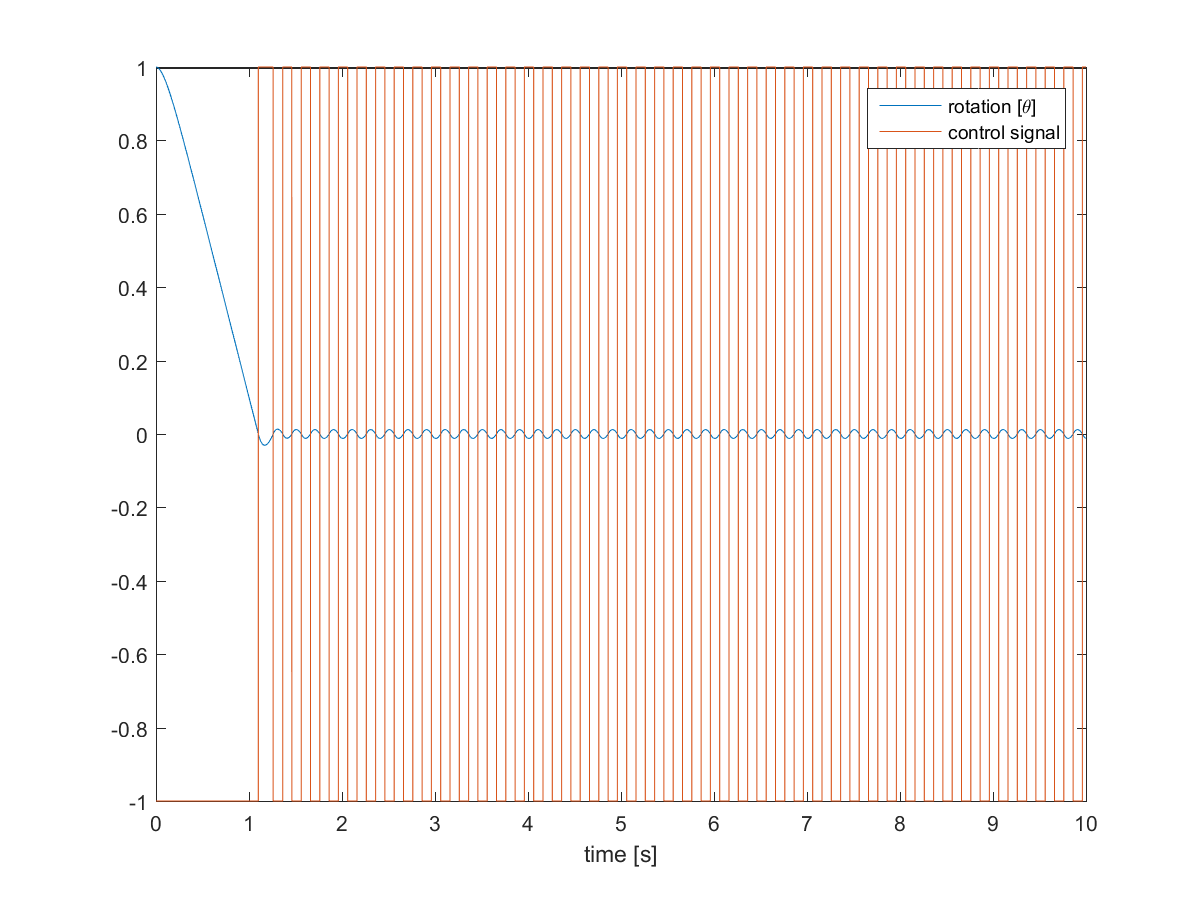
\includegraphics[scale = 0.5, width=1\linewidth]{../matlab/images/task5_plot.png}
        \caption{Response of rot1 simulink model.}
        \label{fig:task5_plot}
    \end{figure}

\section*{Task 6}

Euler forward is a forward difference, in the $z$-transform written as
\begin{equation}
s = \frac{z-1}{T_s},
\end{equation}
where $s$ denotes the Laplace transform and the $z$-transform represents a time shift forward in the discrete domain. Applied to the dynamics of the $x$ variable, one yields
\begin{equation}
\frac{z-1}{T_s}x=Ru_\omega cos(\theta)
\end{equation}
which with similar calculations for all state variables yields the complete discrete system dynamics
\begin{align*}
x[k+h] = x[k] + T_s R u_\omega cos(\theta [k])	\\
y[k+h] = y[k] + T_s R u_\omega sin(\theta [k]) \\
\theta[k+h] = \theta [k] + \frac{T_s R}{L} u_\psi.
\end{align*}

\section*{Task 7}
 	Given
	\begin{equation}
		\dot{\theta} = \frac{Ru_\Psi}{L}
		 \label{eq:thetadot}
	\end{equation}
	and
	\begin{equation}
		u_\Psi{[k]} = K_{\Psi}({\theta}^R  - {\theta}[k]).
	\end{equation}
	With Eueler forward equation~\ref{eq:thetadot} gives
	\begin{equation}
		\theta[k+h] = \dot{\theta}[k]\tau_s + \theta[k]
	\end{equation}
	\begin{equation}
		\theta[k+h] = \frac{RK\tau_s({\theta}^R  - {\theta}[k])}{L} + \theta[k]
	\end{equation}
	\begin{equation}
R2 = R2 + R(1,i)^2;		\theta[k+h] =\theta[k](1-\frac{RK\tau_s}{L}) + \frac{RK_p\theta^R\tau_s}{L}
	\end{equation}
The eigenvalues are
	\begin{equation}
		\lambda = \left|{(1-\frac{RK\tau_s}{L})}\right| < 1
	\end{equation}
	which gives that 
	\begin{equation}
		0 < K < \frac{2L}{R\tau_s}
	\end{equation}

\section*{Task 8}
    The simulated task chosen was to rotate from $\theta = 0$ to $\theta = 90$.
    The angular response can be seen in Figure~\ref{fig:task8_angleplot}. The
    position's response can be seen inFigure~\ref{fig:task8_posplot} and shows
    that the position does not change.  \begin{figure}[H]
        \centering
        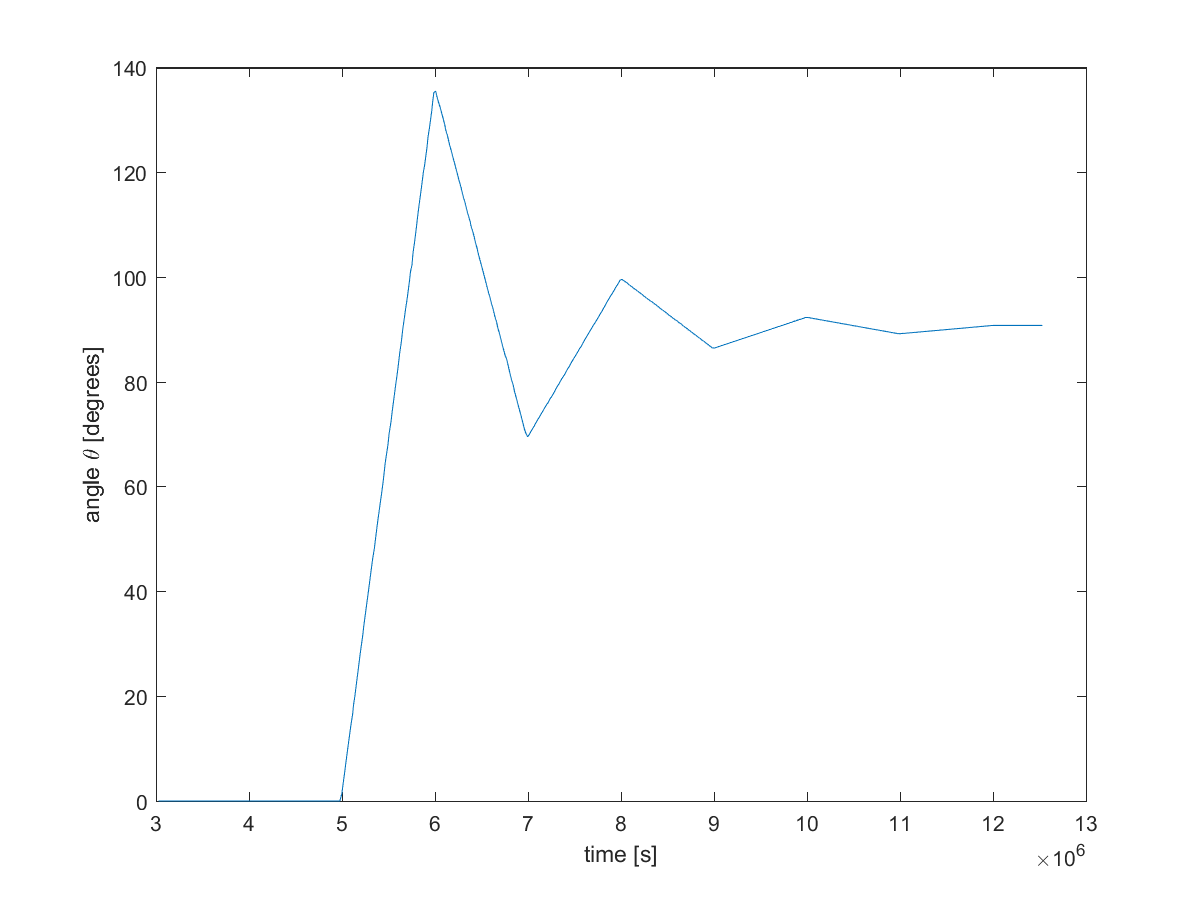
\includegraphics[scale = 0.5]{../matlab/images/task8_angleplot.png}
        \caption{Simulated rotation resonse.}
        \label{fig:task8_angleplot}
    \end{figure}
    \begin{figure}[H]
        \centering
        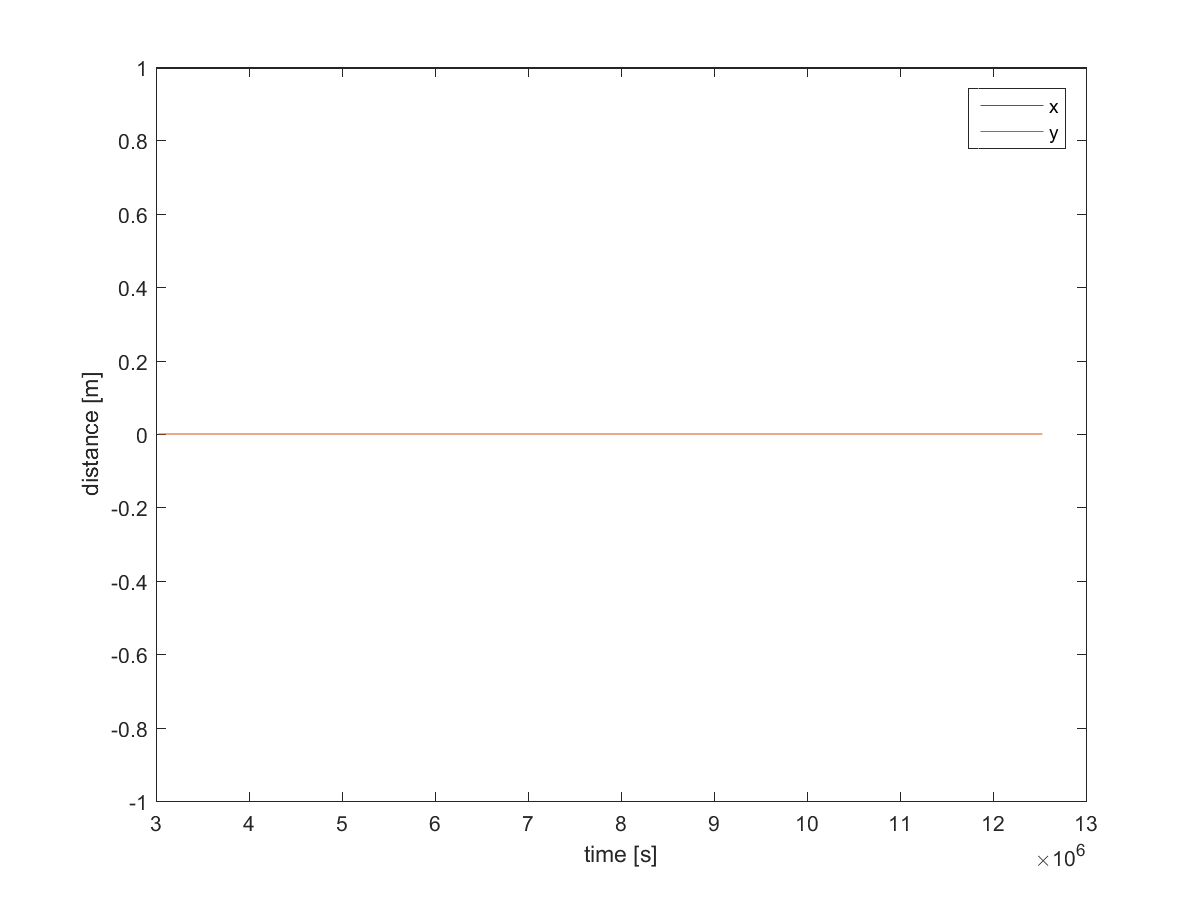
\includegraphics[scale = 0.5]{../matlab/images/task8_posplot.png}
        \caption{Simulated position response.}
        \label{fig:task8_posplot}
    \end{figure}

\section*{Task 9}
plot(x,y)
 	The equation 
	\begin{equation}
		d_0[k] = K_\omega(cos(\frac{\theta[k]\pi}{180}))*(x_0-x[k]) + (sin(\frac{\theta[k]\pi}{180}))*(y_0-y[k])
	\end{equation}
 	describes how $d_0$ changes with time.
\section*{Task 10}
In Figure~\ref{fig:task10_stepplot} the performance of the controller is shown.
Figure~\ref{fig:task10_stepplot} plot(x,y)shows that the controller is able to maintain
its starting position.  \begin{figure}[H]
        \centering
        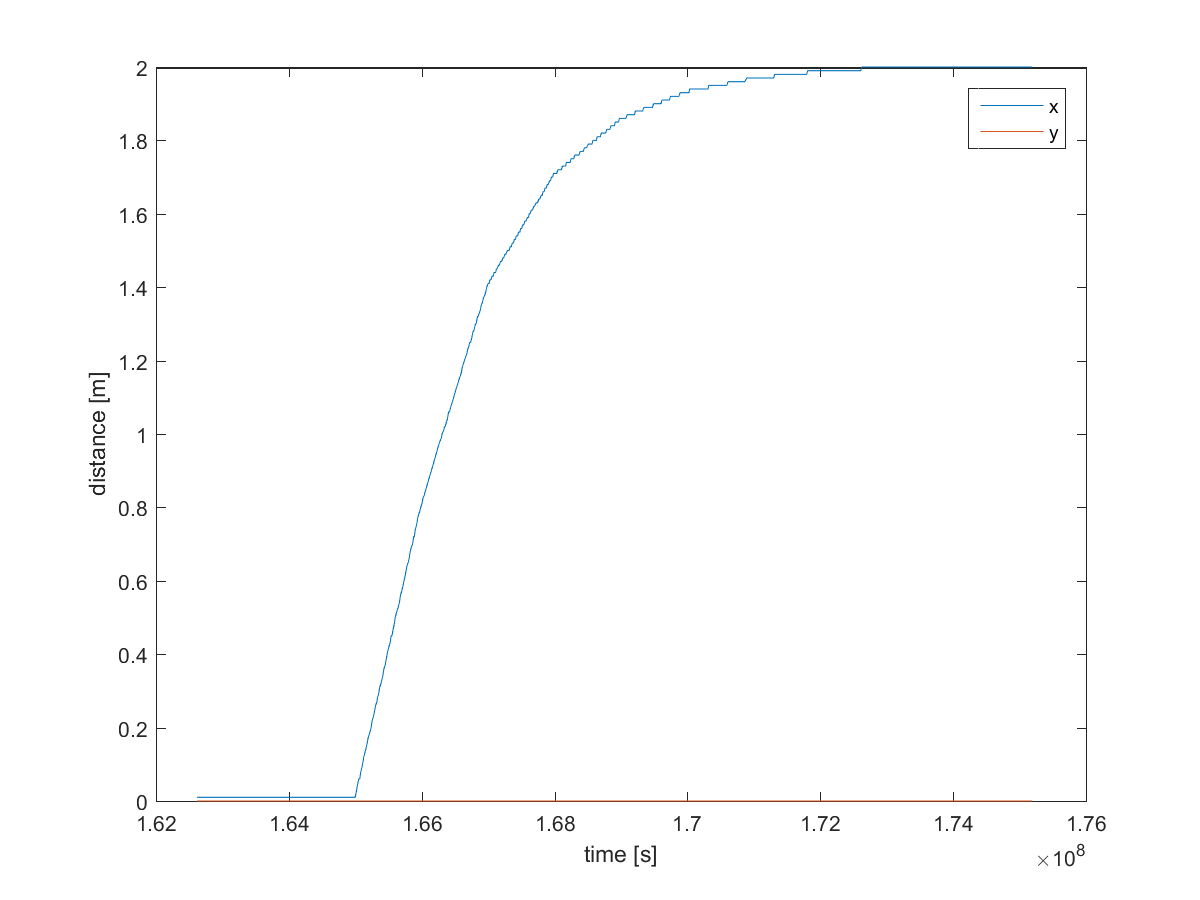
\includegraphics[scale = 0.5]{../matlab/images/task10_stepplot.png}
        \caption{Simulated position response when setting start to a different position.}
        \label{fig:task10_stepplot}
    \end{figure}
    
    \begin{figure}[H]
        \centering
        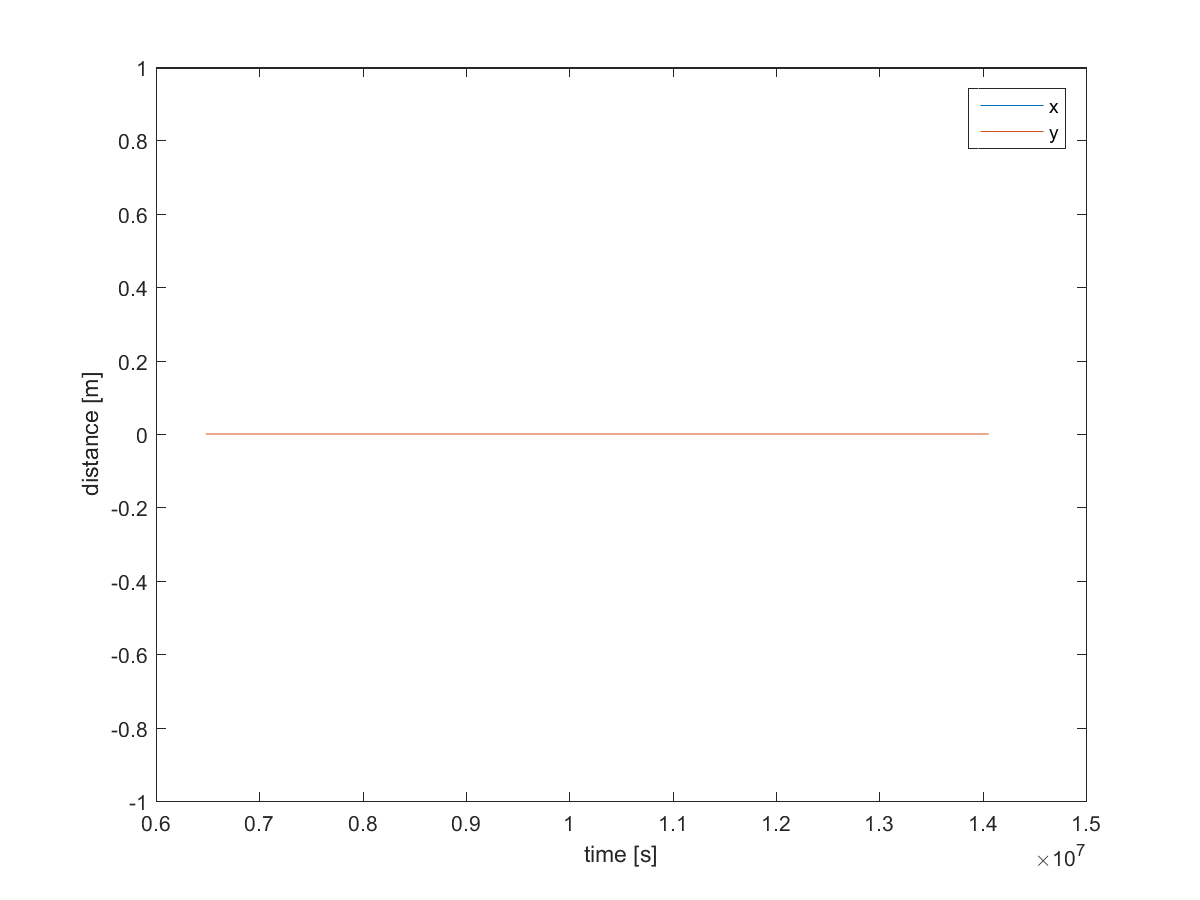
\includegraphics[scale = 0.5]{../matlab/images/task10_stillplot.png}
        \caption{Simulated position response when attempting to stand still.}
        \label{fig:task10_stillplot}
    \end{figure}

\section*{Task 11}
In Figure~\ref{fig:task11_angleplot} the error $\theta^R - \theta[k]$ can be seen. In Figure~\ref{fig:task11_d0plot} $d_0$ can be seen.

\begin{figure}[H]
        \centering
        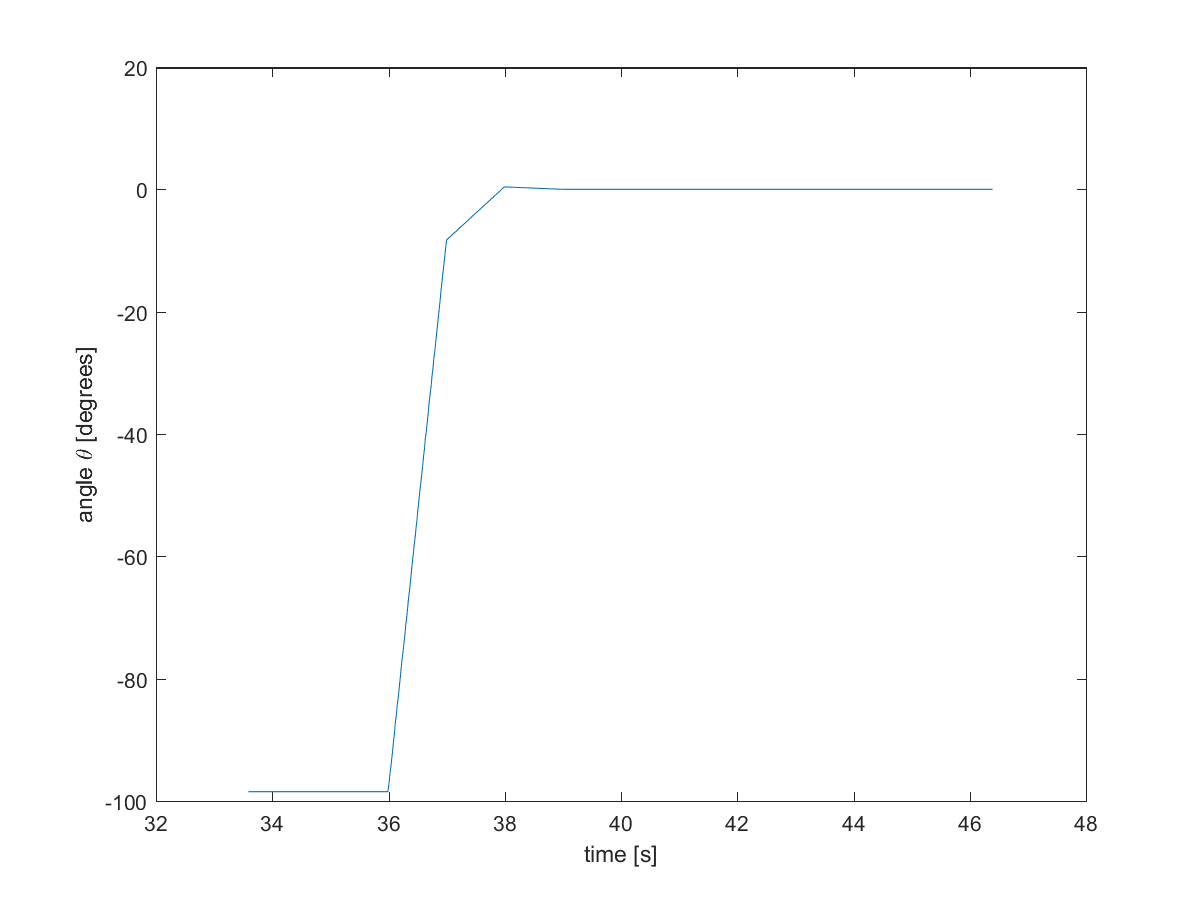
\includegraphics[scale = 0.5]{../matlab/images/task11_angleplot.png}
        \caption{Simulated angular response.}
        \label{fig:task11_angleplot}
    \end{figure}
    
    \begin{figure}[H]
        \centering
        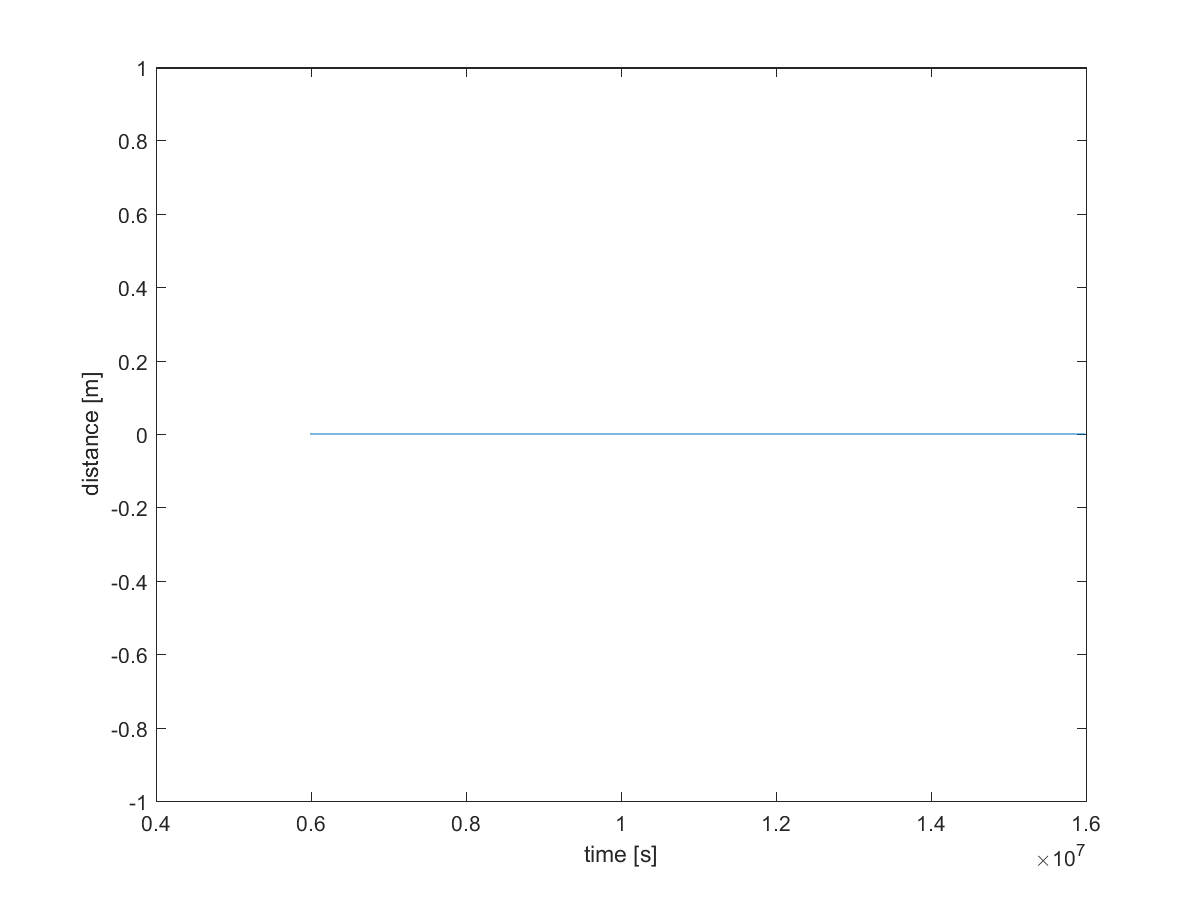
\includegraphics[scale = 0.5]{../matlab/images/task11_d0plot.png}
        \caption{Simulated position response.}
        \label{fig:task11_d0plot}
    \end{figure}

\section*{Task 12}
 	Given
	\begin{equation}
		u_\omega[k]= K_\omega((cos(\theta_g))(x_g-x[k]) + (sin(\theta_g))(y_g-y[k]))
	\end{equation}
	together with
	\begin{equation}
		x[k+1] = x[k]R\tau_scos(\theta[k])u_\omega
	\end{equation}
	\begin{equation}
		y[k+1] = y[k]R\tau_ssin(\theta[k])u_\omega
	\end{equation}
	gives
	\begin{equation}
		x[k+1] = x[k]R\tau_scos(\theta[k])K_\omega((cos(\theta_g))(x_g-x[k]) + (sin(\theta_g))(y_g-y[k]))
		 \label{eq:xkp1}
	\end{equation}
	\begin{equation}
		y[k+1] = y[k]R\tau_ssin(\theta[k])K_\omega((cos(\theta_g))(x_g-x[k]) + (sin(\theta_g))(y_g-y[k]))
		 \label{eq:ykp1}
	\end{equation}
	Looking at the separate stability criteria in both Equation~\ref{eq:xkp1} and~\ref{eq:ykp1} gives
	\begin{equation}
		\lambda-(1-\tau_sRK_{\omega}cos^2(\theta[k])) = 0
	\end{equation}
	\begin{equation}
		\lambda-(1-\tau_sRK_{\omega}sin^2(\theta[k])) = 0
	\end{equation}
	which in turn gives
	\begin{equation}
		\left| (1-\tau_sRK_{\omega}cos^2(\theta[k])) \right | < 1
	\end{equation}
	\begin{equation}
		\left| (1-\tau_sRK_{\omega}sin^2(\theta[k])) \right | < 1
	\end{equation}
	which in turn gives
	\begin{equation}
		K_\omega < \frac{2}{\tau_sRcos^2\theta[k]}
	\end{equation}
	\begin{equation}
		K_\omega < \frac{2}{\tau_sRsin^2\theta[k]}.
	\end{equation}
  	Assuming the worst possible case for theta gives
	%\begin{equation}
	%	0 < K_\plot(x,y)mega < \frac{2}{\tau_sR\theta[k]}.
	%\end{equation}
	A more effective $K_\omega$ is chosen manually through multiple simulations.
\section*{Task 13}

 In figure \ref{fig:task13_positionplot} the position response can be seen.

\begin{figure}[H]
        \centering
        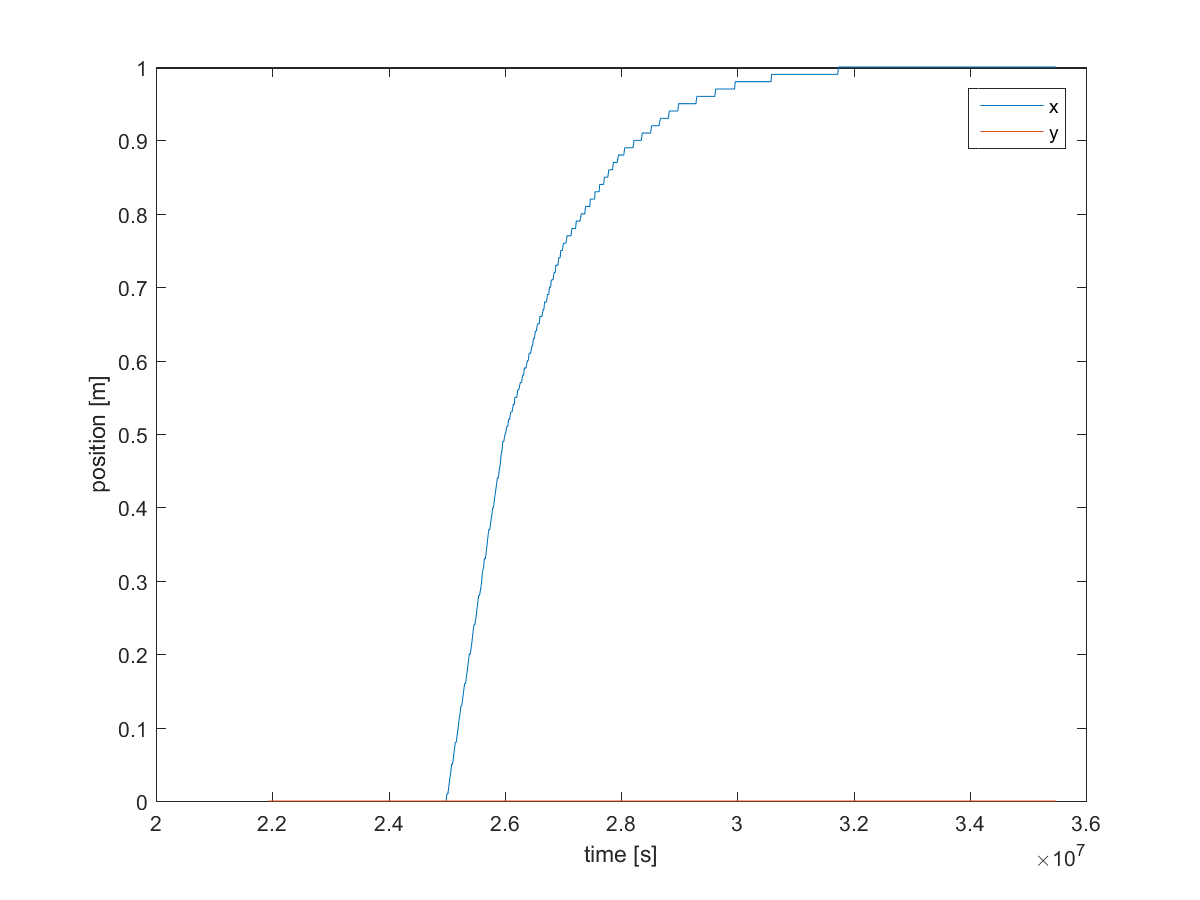
\includegraphics[scale = 0.5]{../matlab/images/task13_positionplot.png}
        \caption{Simulated position response.}
        \label{fig:task13_positionplot}
    \end{figure}

\section*{Task 14}

Solution to the task

\section*{Task 15}

Solution to the task

\section*{Task 16}

Solution to the task

\section*{Task 17}

Solution to the task

\section*{Task 18}

The hybrid automation is defined as,

\begin{equation}
    H = (Q,S,Init,f,D,E,G,R).
\end{equation}
We can model the controller with $Q$, the discrete state space $S$,
the continuous state space and initial states as,
\begin{align*}
    &Q=(Rotation,Translation,Goal)=(q_1,q_2,q_3) \\
    &S=\mathbb{R}^3 (x,y,\theta)\\
    &Init = Q \times \{ S \in \mathbb{R}^3 :x_0\wedge y_0 \wedge
    \theta_0\}
\end{align*} 
the vector fields, $f$ as,
\begin{align*}
    &f(q_1,S)=(Ru_{\omega}cos\theta,Ru_{\omega}sing\theta,R/Lu_{\Psi}) \\
    &f(q_2,S)=(Ru_{\omega}cos\theta,Ru_{\omega}sing\theta,R/Lu_{\Psi})\\
    &f(q_3,S)=(0,0,0),
\end{align*}
the domains, $D$ as,
\begin{align*}
    &D(q_1)=\{S\in \mathbb{R}^3:\theta \le r_1; |(x,y)-(x_0,y_0)|\le r_2\} \\
    &D(q_2)=\{S\in \mathbb{R}^3:|(x,y)-(x_g,y_g)| \le r_2\} \\
    &D(q_3)=\{S\in \mathbb{R}^3:|(x,y)-(x_g,y_g)| \le r_2\}
\end{align*}
the edges, $E$ as,
\begin{align*}
    &E = \{(q_1,q_2), (q_2,q_3), (q_3, q_1)\},
\end{align*}
the guards, $G$ as,

\begin{align*}
    &G_1(q_1,q_2)=\{\theta\in\mathbb{R}:\theta\le r_1\} \\
    &G_2(q_2,q_1)=\{\theta\in\mathbb{R}:\theta\le r_2\} \\
    &G_3(q_3,q_1)=\{Reset\}
\end{align*}
and the resets, $R$ as,
\begin{align*}
  &R(q_1,q_2,S)=R(q_2,q_3,S)=R(q_3,q_1,S)=\{S\}.
\end{align*}


\section*{Task 19}
  The state transitions can be seen in figure \ref{fig:task19_trans}
  where state 0 is rotating, state 1 is translation and state 2 is
  standstill. 

\begin{center}
    \begin{figure}[H]
      \centering
      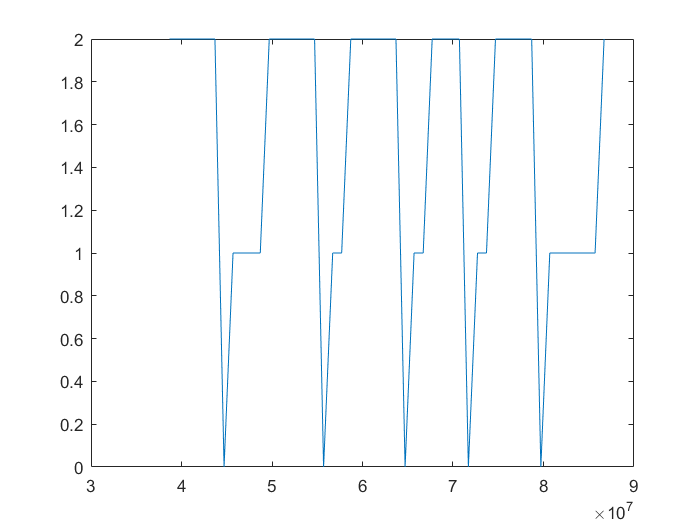
\includegraphics[scale = 0.5]{../matlab/images/task19_trans.png}
      \caption{State transitions for the controller between state 1, 2
      and 3}
      \label{fig:task19_trans}
    \end{figure}
\end{center}

This is when driving 1 $\rightarrow$ 3 $\rightarrow$ 6 $\rightarrow$ 5
$\rightarrow$ 8 $\rightarrow$ 1. This can also be seen in the plot in
figure \ref{fig:task13_positionplot} where the performance of the robot
can be seen.

\begin{center}
    \begin{figure}[H]
      \centering
      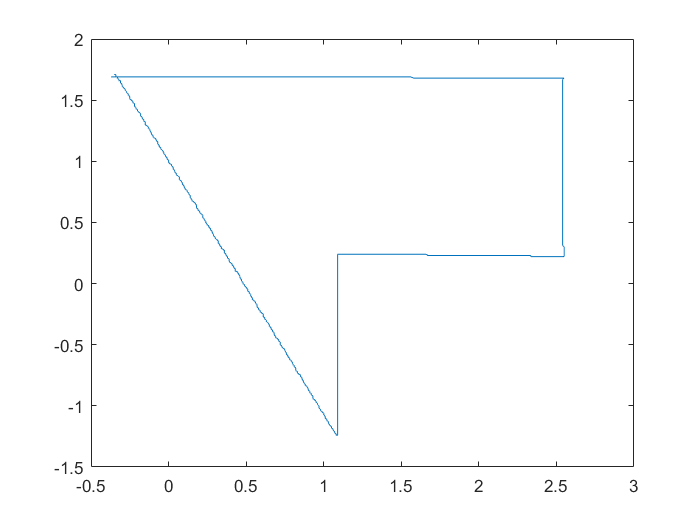
\includegraphics[scale=0.5]{../matlab/images/task19_cont.png}
      \caption{Control performance for the robot}
      \label{fig:task19_cont}
    \end{figure}
\end{center}

\section*{Task 21}

The difficulty comes from the delay between the computer and the
robot. There is a certain delay between when the user presses the button
and the robot responds. 
\section*{Task 22}
G
Solution to the task



%%%%%%%%%%%%%%%%%%%%%%%%%%%%%%%%%%%%%%%%%%%%%%%%%%%%%%%%%%%%%%%%%%%%%%%%%%%%%%%%%%%
% The bibliography
%%%%%%%%%%%%%%%%%%%%%%%%%%%%%%%%%%%%%%%%%%%%%%%%%%%%%%%%%%%%%%%%%%%%%%%%%%%%%%%%%%%
%\bibliography{Bibliography_template} %Read the bibliography from a separate file

\begin{thebibliography}{99}
\bibitem[Khalil(2002)]{Khalil:2002:Nonlinear-systems:vh}
Hassan~K Khalil.
\newblock \emph{Nonlinear systems}.
\newblock Prentice Hall, Upper Saddle river, 3. edition, 2002.
\newblock ISBN 0-13-067389-7.

\bibitem[Oetiker et~al.(2008)Oetiker, Partl, Hyna, and
  Schlegl]{Oetiker:2008:TheNotSoShortIntroductiontoLaTeXe}
Tobias Oetiker, Hubert Partl, Irene Hyna, and Elisabeth Schlegl.
\newblock \emph{The Not So Short Introduction to \LaTeXe}.
\newblock Oetiker, OETIKER+PARTNER AG, Aarweg 15, 4600 Olten, Switzerland,
  2008.
\newblock http://www.ctan.org/info/lshort/.

\bibitem[Sastry(1999)]{Sastry:1999:Nonlinear-systems:-analysis-stability-and-c%
ontrol:xr}
Shankar Sastry.
\newblock \emph{Nonlinear systems: analysis, stability, and control},
  volume~10.
\newblock Springer, New York, N.Y., 1999.
\newblock ISBN 0-387-98513-1.
\end{thebibliography}


\end{document}      % End of the document
